\documentclass[11pt,a4paper]{article}
\usepackage[T1]{fontenc}
\usepackage[utf8]{inputenc}
\usepackage{lmodern,microtype}
\usepackage[margin=25mm,headheight=14pt]{geometry}
\usepackage{amsmath,amssymb,amsthm,mathtools}
\usepackage{booktabs,array,tabularx,longtable,enumitem}
\usepackage{xcolor,tikz,listings,fancyhdr,xurl}
\usetikzlibrary{positioning}
\definecolor{ink}{HTML}{173445}
\definecolor{accent}{HTML}{126765}
\definecolor{quiet}{HTML}{52636D}
\definecolor{shade}{HTML}{F3F6F7}
\definecolor{colorzero}{HTML}{356DA8}
\definecolor{colorone}{HTML}{C37B23}
\definecolor{colortwo}{HTML}{44815C}
\definecolor{colorthree}{HTML}{8A5CA1}
\definecolor{colorfour}{HTML}{B45655}
\usepackage[colorlinks=true,linkcolor=accent,citecolor=accent,urlcolor=accent,
pdfauthor={Keio, with ChatGPT assistance},
pdftitle={Degree Modes and Hard-Edge Log-Concavity: Two Exact Obstruction Arguments}]{hyperref}
\newtheorem{theorem}{Theorem}[section]
\newtheorem{lemma}[theorem]{Lemma}
\newtheorem{proposition}[theorem]{Proposition}
\newtheorem{corollary}[theorem]{Corollary}
\theoremstyle{definition}
\newtheorem{definition}[theorem]{Definition}
\newtheorem{problem}[theorem]{Problem}
\theoremstyle{remark}
\newtheorem{remark}[theorem]{Remark}
\DeclareMathOperator{\girth}{girth}
\DeclareMathOperator{\dist}{dist}
\DeclareMathOperator{\mode}{mode}
\newcommand{\PP}{\mathbb P}
\newcommand{\EE}{\mathbb E}
\newcommand{\Bess}{\operatorname{Bess}}
\newcommand{\HS}{\mathrm{HS}}
\newcommand{\gt}{\gamma_t}
\newcommand{\mmin}{\operatorname{mode}_{\min}}
\newcommand{\N}{N}
\newcommand{\Gstar}{G_{\ast}}
\newcommand{\core}{D_{\ast}}
\newcommand{\VMRC}{\textsc{vmrc}}
\newcommand{\code}[1]{\texttt{#1}}
\setlist{topsep=5pt,itemsep=3pt,parsep=0pt}
\setlength{\emergencystretch}{2em}
\setlength{\parskip}{3pt}
\setlength{\parindent}{1.15em}
\pagestyle{fancy}
\fancyhf{}
\fancyhead[L]{\small\color{quiet}Degree modes and hard-edge log-concavity}
\fancyhead[R]{\small\color{quiet}Keio}
\fancyfoot[C]{\thepage}
\renewcommand{\headrulewidth}{0.3pt}
\lstdefinestyle{python}{
 language=Python,basicstyle=\ttfamily\footnotesize,
 keywordstyle=\color{accent}\bfseries,commentstyle=\color{quiet},
 stringstyle=\color{ink},showstringspaces=false,
 columns=fullflexible,keepspaces=true,breaklines=true,
 frame=single,rulecolor=\color{quiet!35},framesep=5pt,
 xleftmargin=5pt,xrightmargin=5pt,
 aboveskip=9pt,belowskip=9pt,tabsize=4
}
\raggedbottom

\title{\color{ink}\bfseries Degree Modes and\\
Hard-Edge Log-Concavity\\[6pt]
\large A counterexample to Graffiti.pc Conjecture 253\\
and an exact threshold for positive Bessel points}
\author{Keio\\[2pt]\small With ChatGPT assistance}
\date{24 November 2026}

\begin{document}
\maketitle
\thispagestyle{plain}

\begin{abstract}
This manuscript contains two independent obstruction arguments.
The principal result is an explicit twenty-vertex counterexample to
Graffiti.pc Conjecture 253, announced on 23 February 2007. The graph is
simple and connected, has girth five, unique degree mode five, and total
domination number five, contradicting the proposed bound
$\gamma_t\geq1+\operatorname{mode}_{\min}$. Its minimum total dominating
set is unique. A neighborhood injection, a short-cycle attachment
criterion, and a complete adjacency certificate give a direct proof.
An embedded standard-library verifier independently checks the graph.

A separate analytic part proves that every finite positive-labelled
law of the Li--Valk\'o $\operatorname{Bess}_{\beta,a}$ process is
log-concave exactly when $\beta(a+1)\geq1$. Necessity follows from an
explicit small-ball asymptotic, obtained by a shifted Laguerre
factorization and a uniform estimate based on inverse-trace tightness.
The sufficient range is prior work; its exactness was explicitly
posed as a question on 14 November 2026.

All mathematical conclusions are proved with their quantifiers closed.
The two parts are not claimed to arise from one new universal principle.
The original graph catalogue still records Conjecture 253 as open in
its November 2026 PDF. Neither that status entry nor bounded literature
searches certify historical priority. No claim of a historically first
solution or superiority to all earlier corpus results is made.
\end{abstract}

\noindent\textbf{Mathematics Subject Classification (2020).}
05C69, 05C07, 05C38; 60B20, 60G55.

\noindent\textbf{Keywords.}
Total domination; degree mode; girth; Graffiti.pc;
hard edge; Bessel point process; log-concavity.



\clearpage
\tableofcontents
\clearpage
\part{A counterexample to Graffiti.pc Conjecture 253}

\section{The original problem and the conclusion}
\label{sec:problem}

All graphs in this paper are finite, simple, and undirected.
For a graph $G$, write $N_G(v)$ for the open neighborhood of a vertex
$v$, $d_G(v)=|N_G(v)|$ for its degree, and $g(G)$ for its girth.
Acyclic graphs may be assigned girth infinity; our example contains
a cycle, so this convention has no bearing on the result.

A set $D\subseteq V(G)$ is a \emph{total dominating set} if
\[
        N_G(v)\cap D\ne\varnothing\qquad(v\in V(G)).
\]
The condition applies to vertices of $D$ as well as to vertices outside
$D$. The total domination number $\gt(G)$ is the minimum cardinality
of such a set. It is defined whenever $G$ has no isolated vertices.

For each integer $j\ge0$, let
\[
        f_j(G)=|\{v\in V(G):d_G(v)=j\}|,\qquad
        h(G)=\max_{j\ge0}f_j(G).
\]
The \emph{smallest degree mode} is
\[
        \mmin(G)=\min\{j:f_j(G)=h(G)\}.
\]
Thus the mode is a \emph{degree value}, whereas $h(G)$ is its
multiplicity. Keeping these two quantities distinct is essential.

Conjecture 253 of DeLaVi\~na's \emph{Written on the Wall II}
asks whether
\begin{equation}\label{eq:original}
       \gt(G)\ge1+\mmin(G)
\end{equation}
for every simple connected graph $G$ with $g(G)\ge5$.
The catalogue dates the statement to 23 February 2007. Its PDF printed
6 November 2026 gives the statement and
definitions on printed page 147 of 316, and labels it open
\cite[p.~147]{wowii}. The numbering is that of
\emph{Graffiti.pc / Written on the Wall II}, not the older
\emph{Written on the Wall} spectral list.

The same catalogue records that Desormeaux and Henning established
the proposed inequality under the stronger hypothesis $g(G)\ge7$,
and cites their 2016 paper \cite{DH}. We use that entry only as a
documented account of prior scope. No theorem from that paper is an
input to our proof.

\begin{theorem}\label{thm:main}
There is a simple connected graph $\Gstar$ such that
\[
\begin{gathered}
       |V(\Gstar)|=20,\qquad |E(\Gstar)|=32,\qquad g(\Gstar)=5,\\
       \gt(\Gstar)=5,\qquad \mmin(\Gstar)=5.
\end{gathered}
\]
Its degree frequencies are
\[
       (f_1,f_2,f_3,f_4,f_5)=(3,4,4,4,5),
\]
and it has a unique minimum total dominating set.
Consequently Graffiti.pc Conjecture 253 is false.
\end{theorem}

The conclusion is a complete refutation of the universal statement
\eqref{eq:original}. A single graph in the original domain suffices:
it requires the false inequality $5\ge6$. The result is not a claim
that \eqref{eq:original} has been proved with an altered constant or
on a restricted family. In particular, no new invariant replaces the
original degree mode.

The proof proceeds in three parts. First, a neighborhood injection
controls the possible location of high-degree vertices relative to a
total dominating set. Second, an attachment criterion preserves the
exclusion of short cycles. Third, a small exact construction arranges
the required degree frequencies. The certificate in
Appendix~\ref{app:code} checks the resulting graph independently.

\section{A neighborhood injection and a bounded search region}
\label{sec:injection}

\begin{lemma}[Neighborhood injection]\label{lem:injection}
Let $G$ have no triangles or four-cycles, and let $D$ be a total
dominating set with $|D|=k$. For every $v\notin D$,
\begin{equation}\label{eq:injection}
        d_G(v)+|N_G(v)\cap D|\le k.
\end{equation}
In particular, $d_G(v)\le k-1$.
\end{lemma}

\begin{proof}
For each $u\in N_G(v)$, choose a vertex
$\phi(u)\in N_G(u)\cap D$, which exists because $D$ totally dominates
$G$. If $\phi(u)\in N_G(v)$, then $v,u,\phi(u)$ form a triangle.
These three vertices are distinct: $\phi(u)\ne u$ because the
neighborhood is open, and $\phi(u)\ne v$ because $v\notin D$.
Therefore $\phi(u)\in D\setminus N_G(v)$.

If distinct vertices $u,u'\in N_G(v)$ have
$\phi(u)=\phi(u')=d$, then
\[
                 v-u-d-u'-v
\]
is a four-cycle. The vertices are again distinct. Thus $\phi$ is
an injection from $N_G(v)$ to $D\setminus N_G(v)$, and
\[
             d_G(v)\le k-|N_G(v)\cap D|.
\]
Finally, $|N_G(v)\cap D|\ge1$ since $D$ also dominates $v$.
\end{proof}

\begin{corollary}[Forced vertices]\label{cor:forced}
In the setting of Lemma~\ref{lem:injection}, every vertex of degree
at least $k$ belongs to $D$. Hence, if $G$ has more than $k$ vertices
of degree at least $k$, then $\gt(G)>k$.
\end{corollary}

\begin{proof}
A vertex of degree at least $k$ cannot lie outside $D$ by
Lemma~\ref{lem:injection}. The final assertion follows by counting
the forced vertices.
\end{proof}

This is a direct short-cycle argument. We do not assert that the
injection principle itself is historically new. Its use here is
concrete: it both restricts the search for a counterexample and
certifies the exact total domination number and uniqueness after
the graph has been constructed.

\begin{proposition}[Size bound for a possible failure]\label{prop:size}
Suppose $G$ is a simple connected graph of girth at least five for
which \eqref{eq:original} fails. Put $k=\gt(G)$ and $h=h(G)$.
Then
\begin{equation}\label{eq:size}
        h\le k,\qquad
        |V(G)|\le k+(k-1)(h-1)\le k^2-k+1.
\end{equation}
\end{proposition}

\begin{proof}
Since all quantities are integers, failure of
$k\ge1+\mmin(G)$ means $\mmin(G)\ge k$.
Let $D$ be a minimum total dominating set.
By Corollary~\ref{cor:forced}, every vertex of degree at least $k$
belongs to $D$, so there are at most $k$ such vertices.
One degree value at least $k$ occurs $h$ times, giving $h\le k$.

Each degree $j\in\{1,\ldots,k-1\}$ has frequency at most $h-1$:
frequency $h$ would make the smallest mode less than $k$.
There are no vertices of degree zero. Counting the low-degree
vertices and the at most $k$ high-degree vertices gives
\[
       |V(G)|\le(k-1)(h-1)+k.
\]
Substituting $h\le k$ proves the second bound.
\end{proof}

The proposition is a genuine restriction on all possible
counterexamples with fixed total domination number. It does not
bound $k$ and therefore cannot by itself turn the original infinite
problem into one exhaustive finite search. For the construction
below, $k=h=5$ permits order at most $21$. The example has order
$20$. This proximity is useful in organizing the construction, but
it does not prove that twenty is the minimum counterexample order.

\section{An auxiliary completion problem and an attachment lemma}
\label{sec:attachment}

The original target remains \eqref{eq:original}. The following
auxiliary problem is introduced solely to construct a certificate
against that existing target.

\begin{problem}[Completion around a prescribed total dominating set]
\label{prob:completion}
Given a graph $F$ without isolated vertices, complete it to a graph
$G$ by attaching other vertices so that:
\begin{enumerate}[label=(\roman*)]
\item $G$ has no triangles or four-cycles;
\item $V(F)$ is a total dominating set of $G$;
\item every vertex of $F$ has a prescribed degree $r$;
\item the degree $r$ occurs more often than every smaller degree.
\end{enumerate}
When $r\ge |V(F)|$, can such a completion be found?
\end{problem}

The question separates three constraints that otherwise interact:
the absence of short cycles, the existence of a small dominating
set, and a strict frequency imbalance in the degree sequence.
Theorem~\ref{thm:main} will answer the auxiliary problem with
$F=P_5$ and $r=5$, then apply that answer to the unchanged
Conjecture 253. The auxiliary problem itself is not counted as an
independent pre-existing problem.

\begin{lemma}[Single-attachment criterion]\label{lem:attachment}
Let $F,H$ be vertex-disjoint simple graphs without triangles or
four-cycles, and let $c:V(H)\to V(F)$ be a map. Form $J$ by adding
the edges $v\,c(v)$ for all $v\in V(H)$. Suppose that:
\begin{enumerate}[label=(\alph*)]
\item for every $uv\in E(H)$, the vertices $c(u)$ and $c(v)$ are
distinct and nonadjacent in $F$;
\item distinct vertices of $H$ with the same image under $c$ have
no common neighbor in $H$.
\end{enumerate}
Then $J$ has no triangles or four-cycles.
\end{lemma}

\begin{proof}
A cycle lying entirely in $F$ or $H$ is already excluded.
A triangle with one vertex in $F$ would use an edge $uv$ of $H$
with $c(u)=c(v)$, contrary to (a). A triangle with two vertices in
$F$ would require a vertex of $H$ to have two neighbors in $F$,
whereas every such vertex has exactly one.

Consider a four-cycle meeting both graphs. If it has exactly one
vertex in $F$, it contains a path $u-w-v$ in $H$ with
$c(u)=c(v)$, contrary to (b). If it has two consecutive vertices
in $F$, its other two vertices form an edge of $H$ whose images
are adjacent in $F$, contrary to (a). If its two vertices in $F$
alternate with its two vertices in $H$, an $H$ vertex has two
neighbors in $F$, which is impossible. The case of three vertices
in $F$ fails for the same reason. These cases exhaust all possible
four-cycles.
\end{proof}

\begin{lemma}[Connectors and leaves]\label{lem:connectors}
In the setting of Lemma~\ref{lem:attachment}, choose distinct
unordered pairs $\{a_i,b_i\}\subseteq V(F)$ such that
$\dist_F(a_i,b_i)\ge3$; vertices in different components have
distance infinity. Add mutually nonadjacent new vertices $z_i$
with
\[
                  N(z_i)=\{a_i,b_i\}.
\]
The resulting graph has no triangles or four-cycles.
Adding arbitrary pendant leaves also preserves this property.
\end{lemma}

\begin{proof}
Add the connector vertices one at a time.
A triangle or four-cycle first created by $z_i$ would require an
existing $a_i$--$b_i$ path of length one or two. No such path lies
in $F$ by the distance assumption. A vertex in $H$ cannot be an
intermediate vertex of a path of length two because it has only
one neighbor in $F$. A previously added connector could be such
an intermediate vertex only if it had the same unordered
neighbor pair, which is excluded. Thus no short cycle is created.
A pendant vertex belongs to no cycle.
\end{proof}

If $F$ has no isolated vertices, every vertex of $F$ has a neighbor
in $F$. Every other vertex introduced by these two lemmas has a
neighbor in $F$, provided the additional leaves are attached to
$F$. Hence $V(F)$ is automatically a total dominating set.
This yields a practical construction rule: first satisfy the two
local conditions on the attachment map, then balance the degrees
with long-distance connectors and leaves.

\section{The twenty-vertex construction}
\label{sec:construction}

Let $F$ be the path
\[
                     a_0-a_1-a_2-a_3-a_4.
\]
Take a disjoint graph $H$ on the ten vertices
\[
                     x,y,p,q,r,s,t,u,w,z.
\]
Its edges are precisely those in the three internally disjoint
$x$--$y$ paths
\begin{equation}\label{eq:theta}
          x-p-y,\qquad x-q-r-y,\qquad x-s-t-u-y,
\end{equation}
together with $sw$ and $uz$. Thus $H$ is
$\Theta(2,3,4)$ with a leaf at $s$ and a leaf at $u$.
The path lengths in the theta notation are numbers of edges.

Define $c$ by Table~\ref{tab:attachments} and add
$v\,c(v)$ for each $v\in V(H)$.
Then add three new leaves $\ell_0,\ell_2,\ell_4$ at
$a_0,a_2,a_4$, respectively. Finally add vertices $b,c$ with
\begin{equation}\label{eq:connectors}
              N(b)=\{a_0,a_3\},\qquad
              N(c)=\{a_1,a_4\}.
\end{equation}
There are no additional edges. Denote the resulting graph by
$\Gstar$.

\begin{table}[htbp]
\centering
\caption{Attachments from $H$ to the five-vertex core.}
\label{tab:attachments}
\begin{tabular}{@{}cccl@{}}
\toprule
Core vertex & Vertices mapped to it & Extra leaf & Connector neighbors\\
\midrule
$a_0$ & $x,u$ & $\ell_0$ & $b$\\
$a_1$ & $r,w$ & none & $c$\\
$a_2$ & $p,t$ & $\ell_2$ & none\\
$a_3$ & $q,z$ & none & $b$\\
$a_4$ & $y,s$ & $\ell_4$ & $c$\\
\bottomrule
\end{tabular}
\end{table}

\begin{figure}[htbp]
\centering
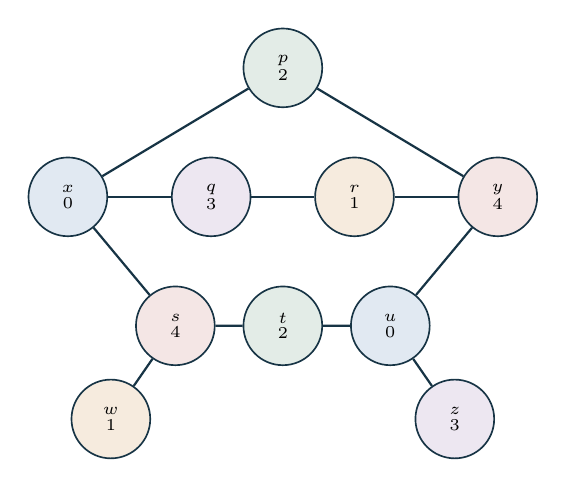
\begin{tikzpicture}[
  scale=0.91,
  vertex/.style={circle,draw=ink,line width=.6pt,minimum size=10mm,
                 inner sep=1.5pt,font=\small},
  edge/.style={draw=ink,line width=.8pt}
]
\node[vertex,fill=colorzero!15] (x) at (-3,0) {$\begin{smallmatrix}x\\0\end{smallmatrix}$};
\node[vertex,fill=colorfour!15] (y) at (3,0) {$\begin{smallmatrix}y\\4\end{smallmatrix}$};
\node[vertex,fill=colortwo!15] (p) at (0,1.8) {$\begin{smallmatrix}p\\2\end{smallmatrix}$};
\node[vertex,fill=colorthree!15] (q) at (-1,0) {$\begin{smallmatrix}q\\3\end{smallmatrix}$};
\node[vertex,fill=colorone!15] (r) at (1,0) {$\begin{smallmatrix}r\\1\end{smallmatrix}$};
\node[vertex,fill=colorfour!15] (s) at (-1.5,-1.8) {$\begin{smallmatrix}s\\4\end{smallmatrix}$};
\node[vertex,fill=colortwo!15] (t) at (0,-1.8) {$\begin{smallmatrix}t\\2\end{smallmatrix}$};
\node[vertex,fill=colorzero!15] (u) at (1.5,-1.8) {$\begin{smallmatrix}u\\0\end{smallmatrix}$};
\node[vertex,fill=colorone!15] (w) at (-2.4,-3.1) {$\begin{smallmatrix}w\\1\end{smallmatrix}$};
\node[vertex,fill=colorthree!15] (z) at (2.4,-3.1) {$\begin{smallmatrix}z\\3\end{smallmatrix}$};
\draw[edge] (x)--(p)--(y);
\draw[edge] (x)--(q)--(r)--(y);
\draw[edge] (x)--(s)--(t)--(u)--(y);
\draw[edge] (s)--(w);
\draw[edge] (u)--(z);
\end{tikzpicture}
\caption{The exterior graph $H$. The lower label $i$ in each vertex
means that this vertex is attached to $a_i$ in the core path.
The drawing shows $H$ only; Table~\ref{tab:attachments} and
\eqref{eq:connectors} specify the remaining edges of $\Gstar$.}
\label{fig:theta}
\end{figure}

\subsection{Order, size, and connectedness}

There are five core vertices, ten vertices in $H$, three additional
leaves, and two connectors. Hence $|V(\Gstar)|=20$.
The edge count is
\begin{equation}\label{eq:sizegraph}
 |E(\Gstar)|=
 \underbrace{4}_{F}+
 \underbrace{11}_{H}+
 \underbrace{10}_{\text{single attachments}}+
 \underbrace{3}_{\text{new leaves}}+
 \underbrace{4}_{\text{connectors}}
 =32.
\end{equation}
The five core vertices form a connected path, and every other vertex
has a neighbor on that path. Thus $\Gstar$ is connected.
Every edge is specified between distinct vertices and appears once,
so the graph is simple.

\subsection{Absence of short cycles}

The core $F$ is a tree. In $H$, every cycle belongs to the theta
subgraph and uses two of the paths in \eqref{eq:theta}; its possible
lengths are $2+3$, $2+4$, and $3+4$. Thus $H$ has no triangles
or four-cycles.

For the attachment map, the absolute differences of color indices
along the three paths in \eqref{eq:theta} are, respectively,
\[
                 (2,2),\qquad (3,2,3),\qquad (4,2,2,4).
\]
The edges $sw$ and $uz$ each have color difference three.
Consequently adjacent vertices of $H$ have distinct,
nonconsecutive colors, as required in condition (a) of
Lemma~\ref{lem:attachment}.

The five pairs of same-color vertices and their neighborhoods in
$H$ are listed in Table~\ref{tab:neighborhoods}. Every pair has
disjoint neighborhoods. This verifies condition (b) directly.

\begin{table}[htbp]
\centering
\caption{The complete check for pairs with a common attachment.}
\label{tab:neighborhoods}
\begin{tabular}{@{}ccc@{}}
\toprule
Pair & First neighborhood in $H$ & Second neighborhood in $H$\\
\midrule
$(x,u)$ & $\{p,q,s\}$ & $\{t,y,z\}$\\
$(r,w)$ & $\{q,y\}$ & $\{s\}$\\
$(p,t)$ & $\{x,y\}$ & $\{s,u\}$\\
$(q,z)$ & $\{x,r\}$ & $\{u\}$\\
$(y,s)$ & $\{p,r,u\}$ & $\{x,t,w\}$\\
\bottomrule
\end{tabular}
\end{table}

Lemma~\ref{lem:attachment} excludes triangles and four-cycles before
the connectors and leaves are added. In $F$,
\[
           \dist_F(a_0,a_3)=\dist_F(a_1,a_4)=3,
\]
and the two connector pairs are distinct. Lemma~\ref{lem:connectors}
therefore applies to $b,c$ and the three leaves.
It follows that $g(\Gstar)\ge5$.
The sequence
\[
                    a_0-a_1-a_2-a_3-b-a_0
\]
is a five-cycle with five distinct vertices. Hence
\begin{equation}\label{eq:girth}
                          g(\Gstar)=5.
\end{equation}

\subsection{The degree census}

The degrees are determined directly by the construction:
\[
\begin{array}{c|l|c}
\text{degree}&\text{vertices}&\text{frequency}\\ \hline
1&\ell_0,\ell_2,\ell_4&3\\
2&w,z,b,c&4\\
3&p,q,r,t&4\\
4&x,y,s,u&4\\
5&a_0,a_1,a_2,a_3,a_4&5
\end{array}
\]
For example, $a_0$ has its one path neighbor, two neighbors
$x,u$ in $H$, the leaf $\ell_0$, and the connector $b$.
The internal core vertex $a_2$ has two path neighbors,
two neighbors $p,t$ in $H$, and the leaf $\ell_2$.
The other three core degrees are checked in the same way using
Table~\ref{tab:attachments}.

The sum of the degrees is
$3+8+12+16+25=64=2\cdot32$, in agreement with
\eqref{eq:sizegraph}. Degree five has strictly greater frequency
than every other degree, so
\begin{equation}\label{eq:mode}
                        \mmin(\Gstar)=5.
\end{equation}
There is no ambiguity about choosing the smallest or largest mode.

\subsection{Exact total domination and uniqueness}

Let
\[
                       \core=\{a_0,a_1,a_2,a_3,a_4\}.
\]
Its induced path has no isolated vertices, so every vertex of
$\core$ has a neighbor in $\core$. Every vertex outside $\core$
was explicitly attached to at least one core vertex.
Thus $\core$ is a total dominating set and $\gt(\Gstar)\le5$.

Suppose there were a total dominating set $D$ of size $k\le4$.
The five core vertices all have degree five, hence degree at
least $k$. Corollary~\ref{cor:forced} would place all five in $D$,
which is impossible. Therefore $\gt(\Gstar)=5$.

If $D$ is any total dominating set of size five, the same corollary
forces every degree-five vertex into $D$. These are precisely the
five vertices of $\core$, so $D=\core$.
This proves uniqueness and completes the proof of
Theorem~\ref{thm:main}.

\section{How the construction was obtained and what was transferred}
\label{sec:method}

\subsection{From the original conjecture to a completion instance}

The construction was found by asking for a small total dominating
set first. Setting $k=5$ in Proposition~\ref{prop:size} suggests
looking at at most twenty-one vertices if the most frequent degree
is at least five. We prescribed the core $P_5$, required every core
degree to be five, and required each degree below five to occur
fewer than five times.

These conditions are neither a change of the original constant nor
a replacement of the original invariant. Any graph satisfying them
and the girth restriction has $\gt(G)\le5$ and
$\mmin(G)=5$, hence refutes \eqref{eq:original}. The auxiliary
completion problem therefore supplies a sufficient \emph{construction
target}; the completed explicit graph supplies the actual refutation.
Stopping at the sufficient target would not have resolved the
conjecture.

A Boolean constraint search was used to discover a candidate edge
set. The constraints enforced a total dominating core, the degree
frequencies, and the exclusion of triangles and four-cycles.
After discovery, the exterior graph was recognized as the theta
configuration in Figure~\ref{fig:theta}. This recognition removed
any need to trust a solver output: the final proof uses only the
explicit construction and the two elementary attachment lemmas.

The neighborhood injection is also what makes the domination
certificate stronger than a mere upper bound. The construction
alone gives $\gt\le5$, which already suffices for the disproof.
The forced-vertex argument adds $\gt=5$ and uniqueness without an
exhaustive search over subsets.

\subsection{Corpus provenance and the extent of the review}

The motivating corpus was the \emph{Verifiable Mathematical
Reasoning Corpus} at the fixed Git commit
\begin{center}
\small\ttfamily
52c1e4ae1f82bd3fdc8b809b9a94e2e4c6ef4cb3.
\end{center}
At that snapshot, 256 top-level \code{.tex} files were retrieved
and searched. The archive numbered [228] was not inspected
internally. Retrieval and text searching do not amount to a
line-by-line validation of all corpus proofs.

The portions directly relevant to this work were the treatment of
degree frequencies and explicit graph counterexamples in [065],
including its Conjecture 369 example; the distinction between
completed arguments and residual conditions in [066]; and the
degree- and distance-multiplicity constructions in [243]
\cite{vmrc065,vmrc066,vmrc243}. These are research manuscripts in
the user's corpus. They were consulted for proof organization and
construction ideas, not assumed to be independently established
theorems.

The concrete transfer consists of preserving the original
invariant's definition, designing an exact degree histogram around
a small structural core, and replacing a discovery computation by
an explicit certificate. The local short-cycle constraints led to
the attachment criterion proved here. We do not claim that a
particular earlier corpus theorem logically implies this
counterexample, or that combining unrelated techniques provides
evidence of mathematical novelty.

Targeted searches in the retrieved text did not locate a treatment
of Graffiti.pc 253. Related mode statements in other catalogue
entries are not the same problem. This finding establishes the
scope of the corpus review, not the absence of every possible
mention inside uninspected archives or differently indexed files.

\section{Verification, scope, and the six research conditions}
\label{sec:audit}

There are two independent routes to the numerical properties in
Theorem~\ref{thm:main}. The mathematical route is the construction,
the degree census, the attachment lemmas, and the forced-vertex
argument. The computational route in Appendix~\ref{app:code}
rebuilds the graph from an explicit adjacency table, checks its
basic properties with integer and finite-set operations, and
enumerates all subsets of sizes one through five.

The verifier has been run. It confirms connectedness, twenty
vertices, thirty-two edges, no triangles, at most one common
neighbor for any distinct pair of vertices, the stated degree
histogram, an explicit five-cycle, no total dominating set of
size at most four, and exactly one of size five. It requires only
the Python standard library and does not invoke a solver.
The tests are supplementary evidence; the preceding mathematical
proof stands without them.

\begin{table}[htbp]
\centering
\caption{Assessment against the six requested research conditions.}
\label{tab:gates}
\small
\begin{tabularx}{\linewidth}{@{}p{.07\linewidth}>{\raggedright\arraybackslash}p{.22\linewidth}X@{}}
\toprule
Gate & Requirement & What this manuscript establishes\\
\midrule
G1 & Pre-existing named problem &
The numbered Graffiti.pc 253 statement and its 2007 date are
documented in the original author's catalogue.\\[4pt]
G2 & Original statement retained &
The graph meets the original connectedness and girth hypotheses.
The original total domination number and degree mode are used.\\[4pt]
G3 & Previously unresolved &
The November 2026 source lists the problem as open. This is
documented status evidence, not an exhaustive certification of
all publications and unpublished work.\\[4pt]
G4 & Unconditional complete conclusion &
A finite explicit graph, with a complete analytic verification,
refutes the universal assertion. No conjecture, numerical
approximation, or unsolved sufficient condition is used.\\[4pt]
G5 & Substantive result &
The certificate changes the status of the literal inequality
from a proposed universal bound to a false statement. The
construction is not a coordinate reformulation. The elementary
proof ingredients are not claimed to be historically new.\\[4pt]
G6 & No prior identical resolution &
No identical resolution was found in the bounded searches.
Priority and exhaustive nonduplication are \emph{not certified}.\\
\bottomrule
\end{tabularx}
\end{table}

The source check included the exact problem number, the original
combination of total domination, girth, and minimum degree mode,
and descriptions of possible small counterexamples.
A failed search for an earlier result is not proof that
none exists. The full text of Desormeaux--Henning \cite{DH} was not
available for a complete comparison in this investigation;
bibliographic metadata and the catalogue's account were checked.

Accordingly, the paper claims the correctness of the displayed
counterexample and its unconditional consequences. It does not
claim that all six historical and novelty conditions have been
definitively certified. It also makes no claim of being the first
published solution, of being more important than every existing
corpus result, or of introducing a historically unprecedented
general principle.

\subsection*{Precisely what remains outside the conclusion}

No minimum-order theorem is proved: there may be a counterexample
with fewer than twenty vertices. No assertion is made that
$g\ge6$ suffices for \eqref{eq:original}, or that a counterexample
of girth six exists. Hence the known girth-seven result is not
declared sharp. The example has a unique mode and a unique minimum
total dominating set, but these extra properties are not proposed
as a classification of all counterexamples.

The construction settles the literal yes-or-no assertion in the
negative. Its mathematical content is fully explicit; historical
priority remains a separate question.



\clearpage
\part{An exact hard-edge log-concavity threshold}
\label{part:hardedge}

This part is independent of the graph construction. It is included as
a second complete mathematical result from the same investigation,
with a different provenance and a different priority status.
The pre-existing question is recent, and the known sufficient
parameter range is credited explicitly.

\section{Target, normalization, and statement}


A probability measure $\mu$ on $\mathbb R^d$ is called
\emph{log-concave} if, for compact sets $A,B$ and $0<t<1$,
\[
 \mu((1-t)A+tB)\geq\mu(A)^{1-t}\mu(B)^t.
\]
For a law with full-dimensional support this is equivalent to having
a log-concave density. This measure formulation includes degenerate
weak limits. The standard density characterization, marginal theorem,
and weak-closure property are used below; see \cite{hePrekopa,heBKM}
for the convexity framework and its random-matrix applications.

Fix $\beta>0$ and $a>-1$, and put
\[
 b=\frac\beta2,\qquad \alpha=b(a+1)>0.
\]
For each integer $n\geq1$, let $(X_1,\ldots,X_n)$ have the labelled
Laguerre density
\begin{equation}\label{he:eq:Laguerre}
 \frac1{Z_n(\alpha)}
 \prod_{i=1}^n x_i^{\alpha-1}e^{-b x_i}
 \prod_{1\leq i<j\leq n}|x_j-x_i|^\beta,
 \qquad (x_1,\ldots,x_n)\in(0,\infty)^n.
\end{equation}
Write the order statistics as $X_{(1)}<\cdots<X_{(n)}$.
The Ram\'irez--Rider theorem \cite[Theorem~1]{heRR} gives joint
convergence of every fixed number of the scaled lowest eigenvalues:
\begin{equation}\label{he:eq:RRlimit}
 (nX_{(1)},\ldots,nX_{(k)})
 \ \Longrightarrow\ (\Lambda_0,\ldots,\Lambda_{k-1}),
 \qquad n\longrightarrow\infty.
\end{equation}
The variables on the right are the lowest eigenvalues of their random
hard-edge operator $G_{\beta,a}$ and satisfy $\Lambda_0>0$ almost surely.

In the exact normalization used for $\Bess_{\beta,a}$ in
\cite[Proposition~12]{heLV}, its positive points obey
\begin{equation}\label{he:eq:normalization}
 (R_0,R_1,\ldots)\ \stackrel{d}=\
 (4\sqrt{\Lambda_0},4\sqrt{\Lambda_1},\ldots).
\end{equation}
This identity fixes the meaning of the process throughout the note.
In particular, no assertion about preservation of log-concavity by a
nonlinear square-root map will be used.

\begin{theorem}\label{he:thm:main}
With the above definitions, put
\[
 \kappa_{\beta,\alpha}
 =\frac{b^{2\alpha-1}\Gamma(1+b)}
 {\Gamma(\alpha)\Gamma(\alpha+b)}.
\]
Then
\begin{equation}\label{he:eq:smallLambda}
 \PP(\Lambda_0\leq s)
 \sim \frac{\kappa_{\beta,\alpha}}{\alpha}s^\alpha
 \qquad(s\downarrow0).
\end{equation}
Consequently,
\begin{equation}\label{he:eq:smallR}
 \PP(R_0\leq r)
 \sim
 \frac{b^{2\alpha-1}\Gamma(1+b)}
 {16^\alpha\Gamma(\alpha+1)\Gamma(\alpha+b)}r^{2\alpha}
 \qquad(r\downarrow0).
\end{equation}
\par\begin{samepage}
\noindent The following assertions are equivalent:
\begin{enumerate}
 \item $\beta(a+1)\geq1$;
 \item for every $k\geq1$ and all indices
 $0\leq j_1<\cdots<j_k$, the probability law of
 $(R_{j_1},\ldots,R_{j_k})$ is log-concave;
 \item the probability law of $R_0$ is log-concave.
\end{enumerate}
\end{samepage}
Here log-concavity is stated for probability measures.  No independent
claim that every limiting multivariate law has a Lebesgue density is
needed.
\end{theorem}

The threshold is therefore exactly
\[
 a\geq\frac1\beta-1.
\]
The sufficiency of this range is already stated in
\cite[Proposition~2.9, as described on the release page]{heEP}.
The question listed there asks whether log-concavity fails below it.
The proof below supplies the lower boundary estimate needed for that
negative direction. This is a separate recent question, not an old
named conjecture. For comparison, \cite[Section~3.1]{heBKM} proves
log-concavity for the hard-edge eigenvalues $\Lambda_j$, proportional
to the squared positive points $R_j^2$, in the
range $a>2/\beta-1$. That statement concerns different coordinates
and is not substituted for the positive-point question here.

\section{A minimum-density factorization}

The Laguerre specialization of the Selberg integral gives
\begin{equation}\label{he:eq:Selberg}
 Z_n(\alpha)
 =b^{-n\alpha-bn(n-1)}
 \prod_{j=1}^n
 \frac{\Gamma(1+jb)\Gamma(\alpha+(j-1)b)}{\Gamma(1+b)}.
\end{equation}
For example, \cite[(1.5)]{heJeong} gives the equivalent formula with
exponential rate $1/2$; rescaling each variable gives
\eqref{he:eq:Selberg}.

\begin{lemma}\label{he:lem:factorization}
Let
\[
 C_n=\frac{nZ_{n-1}(\alpha+\beta)}{Z_n(\alpha)}
 =\frac{n b^\alpha\Gamma(1+b)\Gamma(\alpha+nb)}
 {\Gamma(1+nb)\Gamma(\alpha)\Gamma(\alpha+b)}.
\]
For $n\geq2$, let $Y_1,\ldots,Y_{n-1}$ be distributed according to
\eqref{he:eq:Laguerre} with $n-1$ particles and shape parameter
$\alpha+\beta$.  Define
\begin{align}
 q_n(u)
 &=\EE\left[
  \prod_{j=1}^{n-1}\left(1-\frac{u}{nY_j}\right)_+^\beta
 \right],\qquad u\geq0,\label{he:eq:q}
\end{align}
where $v_+=\max(v,0)$.
Then $0\leq q_n\leq1$, and
\begin{equation}\label{he:eq:CDFn}
 \PP(nX_{(1)}\leq s)
 =\frac{C_n}{n^\alpha}
 \int_0^s u^{\alpha-1}e^{-bu/n}q_n(u)\,du,
 \qquad s\geq0.
\end{equation}
Moreover,
\begin{equation}\label{he:eq:Cnlimit}
 \frac{C_n}{n^\alpha}\longrightarrow\kappa_{\beta,\alpha}.
\end{equation}
\end{lemma}

\begin{proof}
Distinguish which one of the $n$ labelled coordinates is minimal and
set its value equal to $t$.  The other coordinates $y_j$ are larger
than $t$, and their interaction with the minimum contributes
\[
 \prod_{j=1}^{n-1}(y_j-t)^\beta
 =\prod_{j=1}^{n-1}y_j^\beta
  \prod_{j=1}^{n-1}(1-t/y_j)^\beta.
\]
The first product changes the shape parameter from $\alpha$ to
$\alpha+\beta$.  Integrating against the resulting normalized
$(n-1)$-particle ensemble gives the minimum density
\[
 f_{X_{(1)}}(t)=C_n t^{\alpha-1}e^{-bt}q_n(nt).
\]
The substitution $u=nt$ proves \eqref{he:eq:CDFn}.
Cancellation in \eqref{he:eq:Selberg} gives the displayed formula for
$C_n$.  Finally,
\[
 \frac{\Gamma(\alpha+nb)}{\Gamma(1+nb)}
 \sim (nb)^{\alpha-1}
\]
gives \eqref{he:eq:Cnlimit}.
\end{proof}

\section{The uniform boundary estimate}

\begin{lemma}\label{he:lem:tight}
For the tilted ensemble in Lemma~\ref{he:lem:factorization}, the variables
\[
 T_n=\sum_{j=1}^{n-1}\frac1{nY_j},\qquad n\geq2,
\]
form a tight family.
\end{lemma}

\begin{proof}
Write $m=n-1$.  The tilted shape is
\[
 \alpha+\beta=b(a+3),
\]
so its hard-edge parameter is $a'=a+2>-1$.
In the construction of \cite[Section~2 and Lemma~6]{heRR}, the nonzero
eigenvalues of
$(K^m_{\beta,a'})^*K^m_{\beta,a'}$ are the reciprocals
$1/(mY_j)$.  Therefore
\[
 T_n=\frac{n-1}{n}\,
       \|K^{n-1}_{\beta,a+2}\|_{\HS}^2.
\]
Ram\'irez and Rider prove that every sequence of these kernels has,
on a suitable coupling, an almost surely Hilbert--Schmidt convergent
subsequence, with an almost surely Hilbert--Schmidt limit.
The norms are therefore tight.  To see the last implication directly,
failure of tightness would give a fixed $\varepsilon>0$ and a
subsequence of norms exceeding a sequence tending to infinity with
probability at least $\varepsilon$.  An almost surely convergent
subsubsequence of finite norms contradicts this.
The factor $(n-1)/n$ preserves tightness.
\end{proof}

\begin{lemma}\label{he:lem:uniform}
For every $\delta\in(0,1)$ there are $C>0$ and $n_0$ such that
\begin{equation}\label{he:eq:uniformq}
 1\geq q_n(u)\geq(1-\delta)e^{-2\beta Cu}
 \quad\text{for }n\geq n_0,\quad0\leq u\leq\frac1{2C}.
\end{equation}
\end{lemma}

\begin{proof}
Choose $C$ and $n_0$ so that
$\PP(T_n\leq C)\geq1-\delta$ for $n\geq n_0$.
On this event, if $u\leq1/(2C)$, then
\[
 0\leq\frac{u}{nY_j}\leq uT_n\leq\frac12
 \quad\text{for every }j.
\]
In particular every positive-part base in \eqref{he:eq:q} is positive.
The elementary bound $\log(1-v)\geq-2v$ for $0\leq v\leq1/2$
gives
\[
 \prod_j\left(1-\frac{u}{nY_j}\right)^\beta
 \geq\exp(-2\beta uT_n)
 \geq e^{-2\beta Cu}.
\]
Taking expectations proves the lower bound.  Every factor in
\eqref{he:eq:q} is at most one, which gives the upper bound.
\end{proof}

\begin{proof}[Proof of the small-ball assertions in Theorem~\ref{he:thm:main}]
Combining \eqref{he:eq:CDFn} and \eqref{he:eq:uniformq} yields, for
$0<s\leq1/(2C)$ and $n\geq n_0$,
\begin{equation}\label{he:eq:sandwich}
 \frac{C_n}{n^\alpha}(1-\delta)
 e^{-bs/n-2\beta Cs}\frac{s^\alpha}{\alpha}
 \leq\PP(nX_{(1)}\leq s)
 \leq\frac{C_n}{n^\alpha}\frac{s^\alpha}{\alpha}.
\end{equation}
The upper bound is valid for every $s\geq0$.

Here is a limit argument requiring no unproved continuity of the
limiting distribution.  By weak convergence in \eqref{he:eq:RRlimit},
the Portmanteau inequality for the open set $(-\infty,t)$ gives
\[
 \PP(\Lambda_0<t)
 \leq\liminf_{n\to\infty}\PP(nX_{(1)}<t)
 \leq\kappa_{\beta,\alpha}\frac{t^\alpha}{\alpha}.
\]
Letting $t\downarrow s$ gives
\[
 \PP(\Lambda_0\leq s)
 \leq\kappa_{\beta,\alpha}\frac{s^\alpha}{\alpha}.
\]
For the lower bound, apply Portmanteau to the closed set $[0,s]$
in \eqref{he:eq:sandwich} and use \eqref{he:eq:Cnlimit}:
\[
 \PP(\Lambda_0\leq s)
 \geq\kappa_{\beta,\alpha}(1-\delta)e^{-2\beta Cs}
             \frac{s^\alpha}{\alpha}.
\]
Divide by $s^\alpha$, first let $s\downarrow0$ with $C$ fixed,
and then let $\delta\downarrow0$.
This proves \eqref{he:eq:smallLambda}.
Substituting $s=r^2/16$ using \eqref{he:eq:normalization} gives
\eqref{he:eq:smallR}.  No moment convergence or uniform integrability
was used: tightness alone controlled the product in \eqref{he:eq:q}.
\end{proof}

\section{The two directions of the threshold}

\begin{lemma}\label{he:lem:lcsmallball}
Let $\mu$ be a nondegenerate log-concave probability measure supported
in $[0,\infty)$.  Then
\[
 \mu([0,r])=O(r)\qquad(r\downarrow0).
\]
\end{lemma}

\begin{proof}
A nondegenerate one-dimensional log-concave measure has a
log-concave density on an interval.  If the left endpoint of its
support is positive, the assertion is immediate.  Otherwise write
this density as $f=e^g$, with $g$ concave on the interior of its
support.  Choose $0<y<z$ in this interior.  For $0<x<y$, set
$\theta=(z-y)/(z-x)$.  Then
$y=\theta x+(1-\theta)z$, whence
\[
 g(x)\leq\frac{g(y)-(1-\theta)g(z)}{\theta}.
\]
For $0<x<y/2$, the parameter $\theta$ stays in a compact subinterval
of $(0,1)$, so the right side is bounded uniformly in $x$.
Thus $f$ is bounded near zero, which gives the assertion.
\end{proof}

\begin{proof}[Proof of the equivalence in Theorem~\ref{he:thm:main}]
Suppose first that $2\alpha=\beta(a+1)\geq1$.
At finite $n$, the ordered singular values
$U_i=\sqrt{X_{(i)}}$ have density proportional to
\begin{equation}\label{he:eq:singulardensity}
 e^{-b\sum_i u_i^2}
 \prod_i u_i^{2\alpha-1}
 \prod_{i<j}(u_j-u_i)^\beta(u_j+u_i)^\beta
\end{equation}
on the convex chamber $0<u_1<\cdots<u_n$.
The exponent $2\alpha-1$ is nonnegative.  The logarithm of
\eqref{he:eq:singulardensity} is consequently a sum of a concave
quadratic and nonnegative multiples of logarithms of positive
affine functions.  It is concave.  Extending the density by zero
off the chamber preserves log-concavity.

By Pr\'ekopa's marginal theorem \cite[Theorem~6]{hePrekopa}, every selected-coordinate marginal
of this density is log-concave.  Positive linear scaling by
$4\sqrt n$ preserves this property.  Equations
\eqref{he:eq:RRlimit} and \eqref{he:eq:normalization} imply that the selected
coordinates converge to the corresponding positive labelled points
of $\Bess_{\beta,a}$.  Log-concave probability measures are closed
under weak limits, so every such limiting law is log-concave.
This proves $(1)\Rightarrow(2)$, and $(2)\Rightarrow(3)$ is immediate.

Finally suppose $2\alpha<1$.  Equation \eqref{he:eq:smallR} implies
\[
 \frac{\PP(R_0\leq r)}r\longrightarrow\infty
 \qquad(r\downarrow0).
\]
It also shows that the law of $R_0$ is nondegenerate: it assigns
positive probability to arbitrarily small positive intervals,
while $R_0>0$ almost surely.
The displayed divergence contradicts Lemma~\ref{he:lem:lcsmallball}
if the law were log-concave.  This proves $(3)\Rightarrow(1)$.
\end{proof}

\section{Checks and scope of the contribution}

As a normalization check, for $(\beta,a)=(2,0)$ one has
$b=\alpha=1$ and $\kappa_{\beta,\alpha}=1$.
The theorem gives $\PP(\Lambda_0\leq s)\sim s$, consistent with the
exact exponential law in this case.  For $(\beta,a)=(1,0)$,
$b=\alpha=1/2$ and $\kappa_{\beta,\alpha}=1/2$, giving
$\PP(\Lambda_0\leq s)\sim\sqrt{s}$.

The central estimate of this note is \eqref{he:eq:uniformq}.  It
turns tightness of a shifted inverse spectral trace into a uniform
lower bound for a whole repulsion product.  An exact density
factorization alone would not justify exchanging the finite-size
limit with the limit toward the hard wall.  The estimate supplies
that missing justification for all $\beta>0$ and $a>-1$, including
parameters for which a first inverse moment need not be finite.

The following priority limitations are essential.
\begin{enumerate}
 \item The positive threshold range was already announced by the
 Evidence Press release \cite{heEP}; it is not a new contribution here.
 \item That release explicitly identified exactness of the range
 as a further question.  It predates this note, but only by ten
 days.  It does not satisfy a preference for a long-standing
 famous conjecture.
 \item Ram\'irez--Rider convergence, the Selberg evaluation,
 Pr\'ekopa marginalization, and weak closure are established tools.
 This proof uses them with their exact normalizations; it does not
 claim to have discovered these tools.
 \item A bounded literature search did not identify a prior theorem
 stated as this exact threshold.  Such a search cannot establish
 priority.  In particular, the small-ball exponent and constant
 may already follow from established hard-edge formulas in some
 or all parameter ranges.  A complete priority audit remains
 necessary before claiming a new research result.
\end{enumerate}


\clearpage
\begin{thebibliography}{99}

\bibitem{wowii}
E.~DeLaVi\~na,
\emph{Written on the Wall II: Conjectures of Graffiti.pc},
Conjecture 253, announced 23 February 2007;
PDF printed 6 November 2026,
p.~147 of 316.
\url{https://www.uhd.edu/academics/sciences/mathematics-statistics/wowii/files/wowiiaii.pdf}.
Catalogue address:
\url{https://cms.uhd.edu/faculty/delavinae/research/wowII/index.htm}.

\bibitem{DH}
W.~J. Desormeaux and M.~A. Henning,
Lower bounds on the total domination number of a graph,
\emph{Journal of Combinatorial Optimization}
\textbf{31} (2016), no.~1, 52--66.
\url{https://doi.org/10.1007/s10878-014-9708-2}.
The girth-seven scope is reported by \cite{wowii};
the full article was not used as a proof input.

\bibitem{vmrc}
QEEDDD,
\emph{Verifiable Mathematical Reasoning Corpus},
Git snapshot
\nolinkurl{52c1e4ae1f82bd3fdc8b809b9a94e2e4c6ef4cb3},
consulted 24 November 2026.
\url{https://github.com/QEEDDD/Verifiable-Mathematical-Reasoning-Corpus/tree/52c1e4ae1f82bd3fdc8b809b9a94e2e4c6ef4cb3}.

\bibitem{vmrc065}
Keio, \emph{Induced Trees, Domination, and Clique Structure in
Graffiti.pc: A consolidated treatment of forty-four WOWII
statements}, seventh expanded edition, 26 October 2026.
\VMRC~[065], \code{WOWII\_Unified.tex}, in \cite{vmrc}.

\bibitem{vmrc066}
Keio, \emph{Proofs, Counterexamples, and Structural Reductions
for Written on the Wall II: An integrated account of Rounds
1--22 with structural extensions}, revised integrated edition,
26 October 2026.
\VMRC~[066], \code{WOWII\_Rounds\_01\_22\_Consolidated.tex},
in \cite{vmrc}.

\bibitem{vmrc243}
\emph{Degree multiplicity and distance in Graffiti graphs:
Inverse degrees, modal distances and coordinates of maximal
independent sets}, research manuscript, 21 November 2026.
\VMRC~[243], \code{Graffiti\_Degree\_Multiplicity\_and\_Distance.tex},
in \cite{vmrc}.


\bibitem{heRR}
J. A. Ram\'irez and B. Rider,
\emph{Diffusion at the random matrix hard edge},
Communications in Mathematical Physics \textbf{288} (2009), 887--906.
\href{https://doi.org/10.1007/s00220-008-0712-1}{doi:10.1007/s00220-008-0712-1}.
\href{https://arxiv.org/pdf/0803.2043}{arXiv:0803.2043}.
Theorem~1 and Lemma~6 are the inputs used here.

\bibitem{heLV}
Y. Li and B. Valk\'o,
\emph{Operator level limit of the circular Jacobi $\beta$-ensemble},
Random Matrices: Theory and Applications \textbf{11} (2022), 2250043.
\href{https://doi.org/10.1142/S2010326322500435}{doi:10.1142/S2010326322500435}.
\href{https://arxiv.org/pdf/2108.11039}{arXiv:2108.11039}.
Proposition~12 fixes the factor $1/16$ in the squared positive points.

\bibitem{heJeong}
S. Jeong,
\emph{The smallest eigenvalue of $\beta$-Laguerre and $\beta$-Jacobi
ensembles and multivariate orthogonal polynomials},
arXiv:2510.04422v2 (2025).
\url{https://arxiv.org/pdf/2510.04422}.
Equation~(1.5) records the Laguerre Selberg normalizer.

\bibitem{hePrekopa}
A. Pr\'ekopa,
\emph{On logarithmic concave measures and functions},
Acta Scientiarum Mathematicarum (Szeged) \textbf{34} (1973), 335--343.
\url{https://rutcor.rutgers.edu/Prekopa/pdf/SCIENT2.pdf}.

\bibitem{heEP}
Evidence Press,
\emph{Log-concavity and positive dependence in Sine-$\beta$ and
Hua--Pickrell processes}, release of 14 November 2026.
\url{https://evidencepress.org/releases/sine-beta-log-concavity/}.
\href{https://doi.org/10.5281/zenodo.24233404}{doi:10.5281/zenodo.24233404}.
The release reports sufficiency in Proposition~2.9 and lists
exactness of the hard-edge threshold as its first further question.
This is a public research release, not a claim here of independent
journal validation.

\bibitem{heBKM}
J. Baslingker, M. Krishnapur and M. Madiman,
\emph{Log-concavity in one-dimensional Coulomb gases and related ensembles},
arXiv:2412.15116v2, 27 January 2026.
\url{https://arxiv.org/abs/2412.15116}.
Section~3.1 discusses weak limits and the squared hard-edge variables.

\end{thebibliography}


\clearpage
\appendix
\section{A complete labeled adjacency certificate}
\label{app:adjacency}

The correspondence between the construction and the integer labels
used in the verifier is
\[
\begin{array}{c|rrrrrrrrrr}
\text{vertex}&a_0&a_1&a_2&a_3&a_4&\ell_0&x&u&w&r\\
\text{label}&0&1&2&3&4&5&6&7&8&9\\ \hline
\text{vertex}&\ell_2&p&t&q&z&b&s&\ell_4&y&c\\
\text{label}&10&11&12&13&14&15&16&17&18&19
\end{array}
\]
Table~\ref{tab:adjacency} specifies every neighborhood. Each
undirected edge appears in two rows; there are thirty-two distinct
edges. This certificate is complete and requires no external graph
file.

\begin{table}[htbp]
\centering
\caption{Adjacency lists for $\Gstar$.}
\label{tab:adjacency}
\begin{tabular}{@{}rll@{}}
\toprule
Label & Construction name & Neighbors\\
\midrule
0 & $a_0$ & $1,5,6,7,15$\\
1 & $a_1$ & $0,2,8,9,19$\\
2 & $a_2$ & $1,3,10,11,12$\\
3 & $a_3$ & $2,4,13,14,15$\\
4 & $a_4$ & $3,16,17,18,19$\\
5 & $\ell_0$ & $0$\\
6 & $x$ & $0,11,13,16$\\
7 & $u$ & $0,12,14,18$\\
8 & $w$ & $1,16$\\
9 & $r$ & $1,13,18$\\
10 & $\ell_2$ & $2$\\
11 & $p$ & $2,6,18$\\
12 & $t$ & $2,7,16$\\
13 & $q$ & $3,6,9$\\
14 & $z$ & $3,7$\\
15 & $b$ & $0,3$\\
16 & $s$ & $4,6,8,12$\\
17 & $\ell_4$ & $4$\\
18 & $y$ & $4,7,9,11$\\
19 & $c$ & $1,4$\\
\bottomrule
\end{tabular}
\end{table}

In these labels the unique minimum total dominating set is
$\{0,1,2,3,4\}$, and a five-cycle is
$(0,1,2,3,15,0)$.
The maximum number of common neighbors of two distinct vertices
is one. This last condition is equivalent to absence of a
four-cycle in any finite simple graph, regardless of whether that
cycle would be induced.

\section{An embedded exact verifier}
\label{app:code}

Save the following listing as a Python file and run it with
Python~3. It uses only \code{collections} and \code{itertools}.
Explicit \code{require} calls raise exceptions on failure, so
verification remains active even under Python's optimization
option \code{-O}. The program both reads the complete adjacency
certificate and independently rebuilds the edge set from the
named construction.

The enumeration checks all subsets of sizes one through five.
There are no total dominating sets of sizes one through four and
exactly one of size five. No enumeration of all graphs, claim of
minimum counterexample order, or solver unsatisfiability
certificate is involved.

\clearpage
\begin{lstlisting}[style=python]
from collections import Counter, deque
from itertools import combinations


def require(condition, message):
    if not condition:
        raise RuntimeError(message)


ADJ = [
    (1, 5, 6, 7, 15),
    (0, 2, 8, 9, 19),
    (1, 3, 10, 11, 12),
    (2, 4, 13, 14, 15),
    (3, 16, 17, 18, 19),
    (0,),
    (0, 11, 13, 16),
    (0, 12, 14, 18),
    (1, 16),
    (1, 13, 18),
    (2,),
    (2, 6, 18),
    (2, 7, 16),
    (3, 6, 9),
    (3, 7),
    (0, 3),
    (4, 6, 8, 12),
    (4,),
    (4, 7, 9, 11),
    (1, 4),
]
n = len(ADJ)
require(n == 20, "wrong order")
adj = [set(row) for row in ADJ]
for v, row in enumerate(ADJ):
    require(len(row) == len(adj[v]), "repeated neighbor")
    require(v not in adj[v], "loop")
    require(all(0 <= u < n for u in row),
            "neighbor out of range")
    for u in row:
        require(v in adj[u], "asymmetric adjacency")

edges = {
    (u, v) for u in range(n) for v in adj[u] if u < v
}
require(len(edges) == 32, "wrong number of edges")

# Rebuild the edge set from the named construction.
named = {
    **{"a" + str(i): i for i in range(5)},
    "l0": 5, "x": 6, "u": 7, "w": 8, "r": 9,
    "l2": 10, "p": 11, "t": 12, "q": 13, "z": 14,
    "b": 15, "s": 16, "l4": 17, "y": 18, "c": 19,
}
rebuilt = set()


def add_edge(a, b):
    u, v = named[a], named[b]
    require(u != v, "construction loop")
    edge = tuple(sorted((u, v)))
    require(edge not in rebuilt, "duplicate construction edge")
    rebuilt.add(edge)


def add_path(*vertices):
    for a, b in zip(vertices, vertices[1:]):
        add_edge(a, b)


add_path("a0", "a1", "a2", "a3", "a4")
add_path("x", "p", "y")
add_path("x", "q", "r", "y")
add_path("x", "s", "t", "u", "y")
add_edge("s", "w")
add_edge("u", "z")
classes = [
    ("a0", ("x", "u")),
    ("a1", ("r", "w")),
    ("a2", ("p", "t")),
    ("a3", ("q", "z")),
    ("a4", ("y", "s")),
]
for core, outside in classes:
    for v in outside:
        add_edge(core, v)
for core, leaf in (("a0", "l0"), ("a2", "l2"),
                   ("a4", "l4")):
    add_edge(core, leaf)
for connector, endpoints in (
    ("b", ("a0", "a3")), ("c", ("a1", "a4"))
):
    for core in endpoints:
        add_edge(connector, core)
require(rebuilt == edges, "construction and certificate differ")

# Connectivity by breadth-first search.
seen = {0}
queue = deque([0])
while queue:
    v = queue.popleft()
    for u in adj[v] - seen:
        seen.add(u)
        queue.append(u)
require(len(seen) == n, "graph disconnected")

# Exact degree histogram and unique mode.
degrees = [len(row) for row in adj]
histogram = Counter(degrees)
require(histogram == {1: 3, 2: 4, 3: 4, 4: 4, 5: 5},
        "wrong degree histogram")
frequency = max(histogram.values())
modes = sorted(d for d, count in histogram.items()
               if count == frequency)
require(modes == [5], "degree mode is not uniquely 5")

# No triangles: adjacent vertices have no common neighbor.
for u, v in edges:
    require(not (adj[u] & adj[v]), "triangle found")

# No 4-cycles, including noninduced cycles.
max_common = max(len(adj[u] & adj[v])
                 for u, v in combinations(range(n), 2))
require(max_common <= 1, "4-cycle found")

# A displayed 5-cycle proves the girth is exactly 5.
cycle = (0, 1, 2, 3, 15)
require(len(set(cycle)) == 5, "cycle repeats a vertex")
for u, v in zip(cycle, cycle[1:] + cycle[:1]):
    require(v in adj[u], "displayed 5-cycle is missing an edge")

# Total domination uses open neighborhoods, also for D itself.
def is_total_dominating(vertices):
    D = set(vertices)
    return all(adj[v] & D for v in range(n))


counts = {}
first_minimum = None
for size in range(1, 6):
    witnesses = [
        D for D in combinations(range(n), size)
        if is_total_dominating(D)
    ]
    counts[size] = len(witnesses)
    if witnesses and first_minimum is None:
        first_minimum = witnesses[0]
require(counts == {1: 0, 2: 0, 3: 0, 4: 0, 5: 1},
        "wrong total-domination census")
require(first_minimum == (0, 1, 2, 3, 4),
        "wrong unique minimum total dominating set")
gamma_t = 5
mode_min = modes[0]
require(gamma_t < 1 + mode_min,
        "the original conjecture is not violated")

print("PASS: n = 20, m = 32, connected, girth = 5")
print("Degree histogram:", dict(sorted(histogram.items())))
print("Unique degree mode:", mode_min)
print("Total-dominating-set counts:", counts)
print("Unique minimum total dominating set:", first_minimum)
print("Conjecture 253 would require 5 >= 6.")
\end{lstlisting}

\noindent The expected final output is:
\begin{lstlisting}[basicstyle=\ttfamily\footnotesize,
frame=single,breaklines=true,columns=fullflexible]
PASS: n = 20, m = 32, connected, girth = 5
Degree histogram: {1: 3, 2: 4, 3: 4, 4: 4, 5: 5}
Unique degree mode: 5
Total-dominating-set counts: {1: 0, 2: 0, 3: 0, 4: 0, 5: 1}
Unique minimum total dominating set: (0, 1, 2, 3, 4)
Conjecture 253 would require 5 >= 6.
\end{lstlisting}



\end{document}
